\section{Experimental results}\label{sec:results}

To give comparative results on the quality of the initialisation processes 
considered in this work, four well-known, categorical, labelled datasets ---
soybean (large), mushroom, breast cancer, and zoo animal --- will be clustered
by the \(k\)-modes algorithm with each of the initialisation processes using
their respective number of classes as the number of clusters. These datasets
have been chosen to fall in line with the established literature, and for their
relative sizes and complexities. Each dataset is openly available under the
\href{http://mlr.cs.umass.edu/ml/}{UCI Machine Learning
Repository}~\cite{Dua2019}, and their characteristics are summarised in
Table~\ref{tab:dataset_summary}.

\begin{table}[htbp]
    \resizebox{\textwidth}{!}{%
        \begin{tabular}{lrrrlrr}
\toprule
{} &  No. rows &  No. cols &  No. classes &  Missing values &  Adjusted no. rows &  Adjusted no. classes \\
\midrule
Breast cancer &       699 &        10 &            2 &            True &                683 &                     2 \\
Mushroom      &      8124 &        22 &            2 &            True &               5644 &                     2 \\
Soybean       &       307 &        35 &           19 &            True &                266 &                    15 \\
Nursery       &     12960 &         8 &            5 &           False &              12960 &                     5 \\
\bottomrule
\end{tabular}

    }\caption{A summary of the benchmark datasets.}\label{tab:dataset_summary}
\end{table}

Clustering algorithms are often evaluated based on their performance as a
classifier~\cite{%
    Arthur2007,Cao2009,Cao2012,Huang1998,Ng2007,Olaode2014,Schaeffer2007%
}. This is a fundamentally flawed approach --- especially given that
classification belongs to an entirely different branch of learning. Moreover,
doing so requires a number of assumptions about the topology of the data within
the metric space that is being considered~\cite{Memoli2011}. One such assumption
is that the classes recorded in the data are indeed separable objects like
clusters.

This analysis does not consider evaluative metrics related to classification
such as accuracy, recall or precision. Instead, only internal measures are
considered such as the cost function defined in~\eqref{eq:cost}. This metric is
label-invariant and its values are comparable across the different
initialisation methods.  Furthermore, the effect of each initialisation method
on the initial and final clusterings can be captured with the cost function. An
additional, and often useful, metric is the silhouette coefficient. This
measures the ratio between the intra-cluster cohesion and inter-cluster
separation of a particular clustering. Therefore, it could be used in a similar
way to reveal the effect of each initialisation method at the beginning and end
of a run of \(k\)-modes.  Unfortunately, this metric loses its intuition under
the distance measure employed here. The remaining performance measures used are
the number of iterations for the \(k\)-modes algorithm to terminate and the time
taken in seconds.

Tables~\ref{tab:breast_cancer_summary}---\ref{tab:zoo_summary} summarise the
results of each initialisation method on the benchmark datasets. Each column
shows the mean value of each metric and its standard deviation in parentheses
over 50 repetitions of the \(k\)-modes algorithm. The data for these results
was generated using the Python library
\href{https://github.com/nicodv/kmodes}{\texttt{kmodes}} in which the proposed
method has been implemented. All of the data included in this paper, and the
code to generate it are archived online~\textcolor{red}{code and data DOI}.

%\begin{definition}\label{def:silhouette}
%    Let \textbf{X} be a dataset and consider a clustering of \textbf{X} into
%    \(k\) parts, denoted by \(C = \left\{C_1, \ldots, C_k\right\}\). For each
%    \(X^{(i)} \in \textbf{X}\), we define the following two quantities:
%    \begin{itemize}
%        \item Let \(a\left(X^{(i)}\right)\) denote the average dissimilarity
%            between \(X^{(i)}\) and every other point in its cluster. Without
%            loss of generality, let \(X^{(i)} \in C_l\). Then:
%            \[
%                a\left(X^{(i)}\right) := \frac{1}{|C_l|} D\left(C_l,
%                X^{(i)}\right)
%            \]
%        \item Let \(b\left(X^{(i)}\right)\) denote the lowest average 
%            dissimilarity between \(X^{(i)}\) and all other points in each
%            cluster other than \(C_l\). That is:
%            \[
%               }b\left(X^{(i)}\right) := \min_{l' \neq l} \left\{
%                \frac{1}{|C_{l'}|} D\left(C_{l'}, X^{(i)}\right) \right\}
%            \]
%    \end{itemize}
%
%With these quantities we define, for each point in our datset, their
%    \emph{silhouette coefficient}, denoted by \(s(X^{(i)})\):
%    \[
%        s(X^{(i)}) := \frac{b\left(X^{(i)}\right) -
%        a\left(X^{(i)}\right)}{\max\left\{a\left(X^{(i)}\right),
%        b\left(X^{(i)}\right)\right\}}
%    \]
%
%    The \emph{silhouette score} of a clustering \(C\) is simply the average of
%all the silhouette coefficients. Silhouette scores take value in the range
%\([-1, 1]\). Negative scores generally suggest that elements in the data have
%been mis-clustered since there exists a closer cluster centre than its own.
%Values around 0 indicate overlapping clusters, whereas silhouette scores close
%to 1 suggest well-separated and effective clusters.
%\end{definition}

\begin{table}
    \centering
    \resizebox{\textwidth}{!}{%
        \begin{tabular}{lllll}
\toprule
{} &      Initial cost &        Final cost & No. iterations &          Time \\
\midrule
Cao      &   2178.00 (0.000) &   1955.00 (0.000) &   4.00 (0.000) &  0.33 (0.010) \\
Huang    &  2123.12 (92.805) &  2023.80 (49.390) &   2.58 (0.810) &  0.23 (0.047) \\
Matching &  2110.68 (87.670) &  2015.42 (40.354) &   2.72 (0.834) &  0.17 (0.022) \\
\bottomrule
\end{tabular}

    }
    \captionof{table}{Summative metric results for the breast cancer dataset
    with \(k=10\).}\label{tab:breast_cancer_summary}\vspace{20pt}

    \resizebox{\textwidth}{!}{%
        \begin{tabular}{lllll}
\toprule
{} &         Initial cost &          Final cost & No. iterations &          Time \\
\midrule
Cao      &     20381.00 (0.000) &    20376.00 (0.000) &   2.00 (0.000) &  5.18 (0.647) \\
Huang    &  23437.06 (1353.506) &  22091.04 (760.220) &   3.06 (1.018) &  5.81 (1.404) \\
Matching &  22970.80 (1264.522) &  21839.24 (753.933) &   2.90 (0.953) &  2.77 (0.300) \\
\bottomrule
\end{tabular}

    }
    \captionof{table}{Summative metric results for the mushroom dataset with
    \(k=4\).}\label{tab:mushroom_summary}\vspace{20pt}

    \resizebox{\textwidth}{!}{%
        \begin{tabular}{llllll}
\toprule
{} &      Initial cost &        Final cost &     Silhouette & No. iterations &          Time \\
\midrule
Cao      &  2220.48 (41.755) &  1423.28 (67.357) &  -0.01 (0.001) &   4.36 (0.898) &  0.69 (0.068) \\
Huang    &  1592.88 (74.713) &  1448.66 (62.399) &  -0.00 (0.001) &   4.20 (1.325) &  0.43 (0.099) \\
Matching &  1586.38 (57.090) &  1327.74 (35.361) &  -0.01 (0.002) &   4.28 (1.031) &  0.23 (0.016) \\
\bottomrule
\end{tabular}

    }
    \captionof{table}{Summative metric results for the soybean dataset with
    \(k=6\).}\label{tab:soybean_summary}\vspace{20pt}

    \resizebox{\textwidth}{!}{%
        \begin{tabular}{lllll}
\toprule
{} &     Initial cost &       Final cost & No. iterations &          Time \\
\midrule
Cao      &   394.00 (0.000) &   284.00 (0.000) &   2.00 (0.000) &  0.04 (0.001) \\
Huang    &  334.44 (31.635) &  309.22 (31.662) &   2.22 (0.648) &  0.03 (0.006) \\
Matching &  342.30 (39.067) &  313.68 (34.028) &   2.32 (0.891) &  0.03 (0.006) \\
\bottomrule
\end{tabular}

    }
    \captionof{table}{Summative metric results for the zoo animal dataset with
    \(k=6\).}\label{tab:zoo_summary}
\end{table}



\begin{figure}
    \centering
    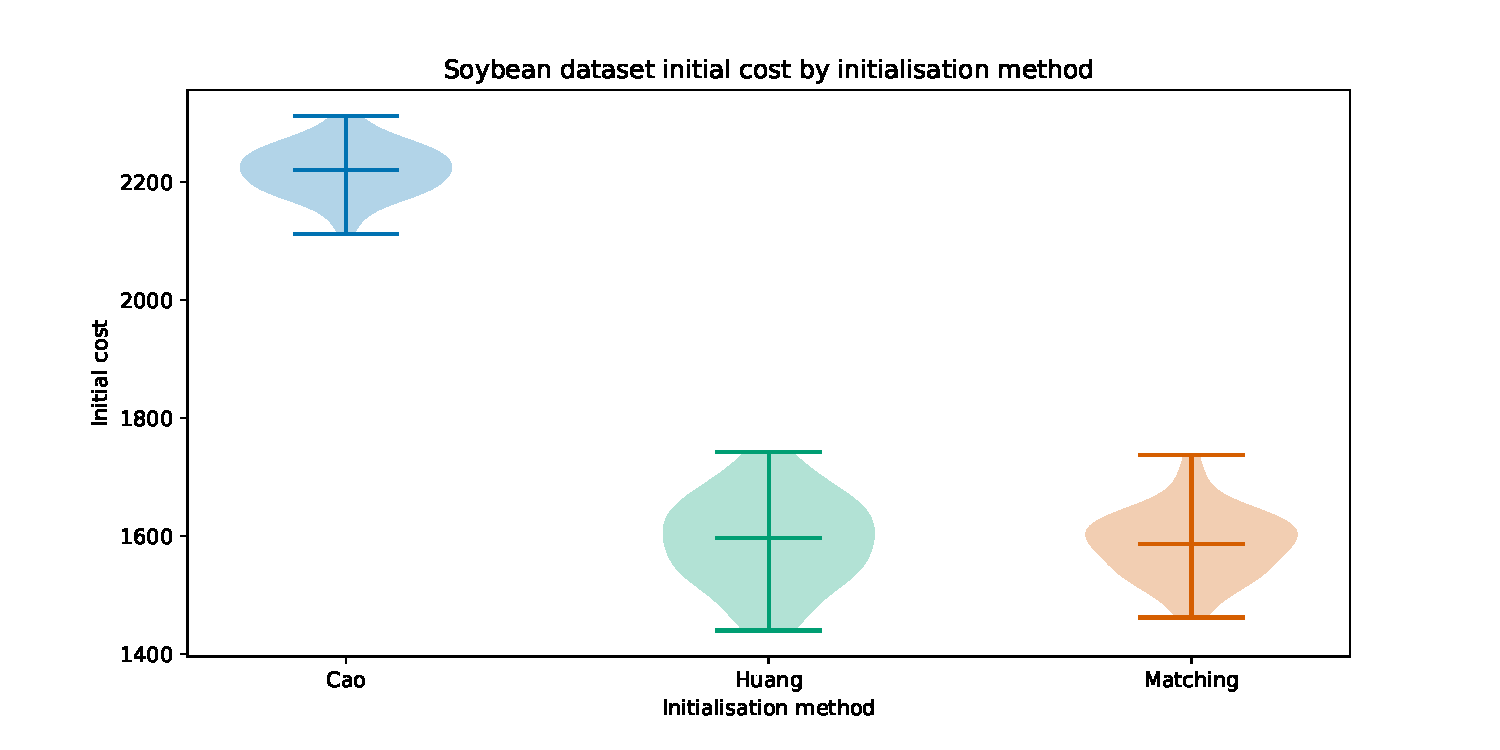
\includegraphics[width=\imgwidth]{%
        img/soybean_initial_cost_violinplot.pdf%
    }\caption{Distribution of initial cost by initialisation for the soybean
              dataset.}
\end{figure}

\begin{figure}
    \centering
    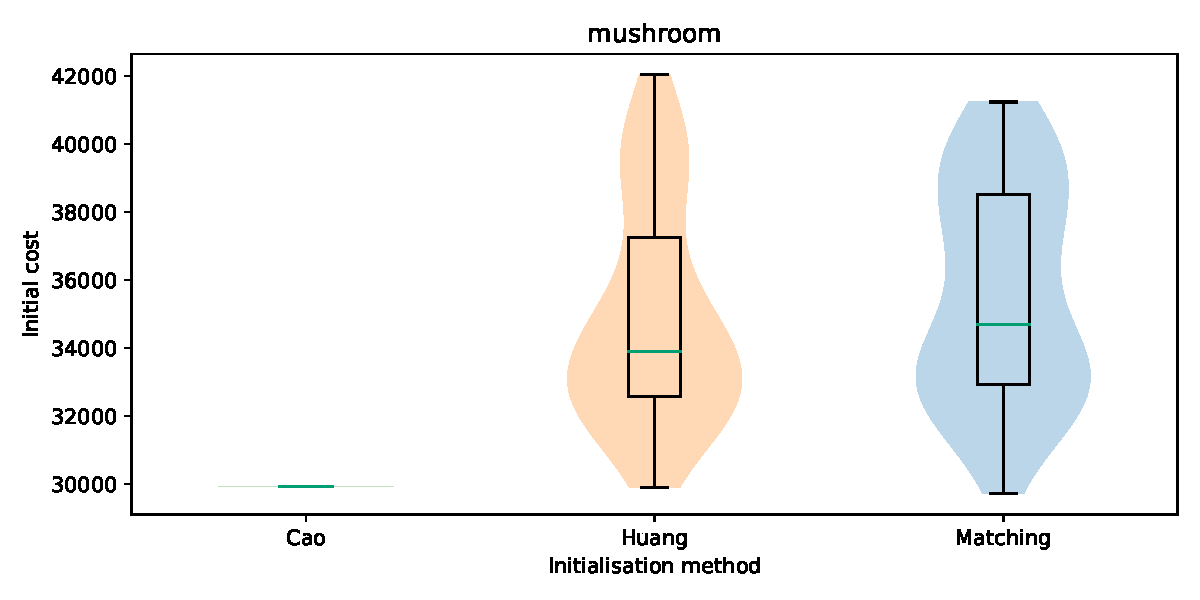
\includegraphics[width=\imgwidth]{%
        img/mushroom_initial_cost_violinplot.pdf%
    }\caption{Distribution of initial cost by initialisation for the mushroom
              dataset.}
\end{figure}

\begin{figure}
    \centering
    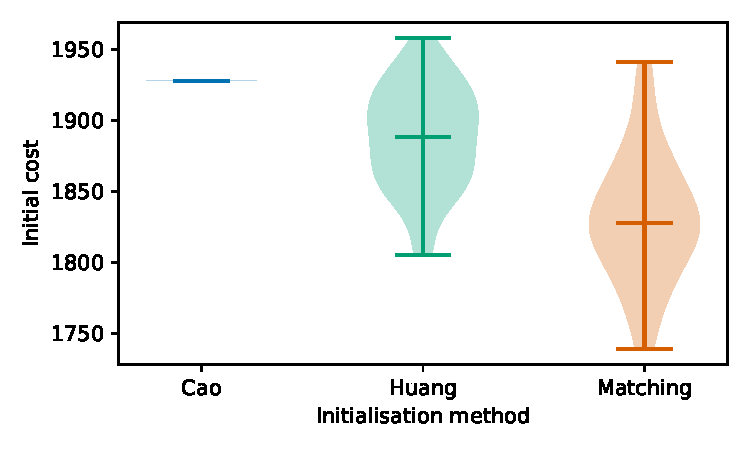
\includegraphics[width=\imgwidth]{%
        img/breast_cancer_initial_cost_violinplot.pdf%
    }\caption{Distribution of initial cost by initialisation for the breast
              cancer dataset.}
\end{figure}

\begin{figure}
    \centering
    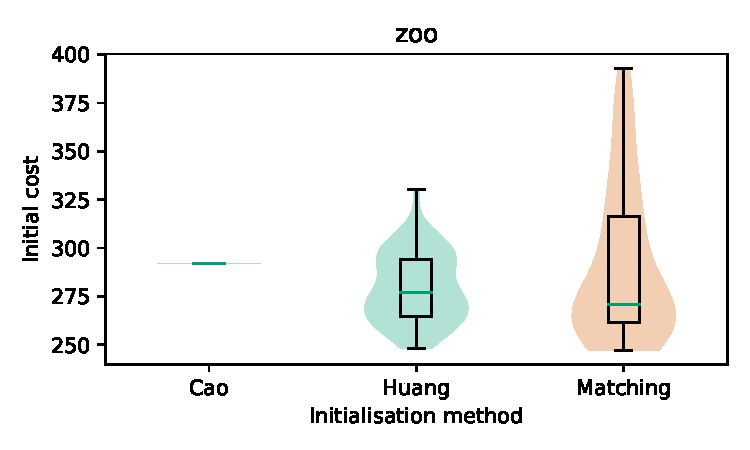
\includegraphics[width=\imgwidth]{%
        img/zoo_initial_cost_violinplot.pdf%
    }\caption{Distribution of initial cost by initialisation for the zoo animal
              dataset.}
\end{figure}


\begin{figure}
    \centering
    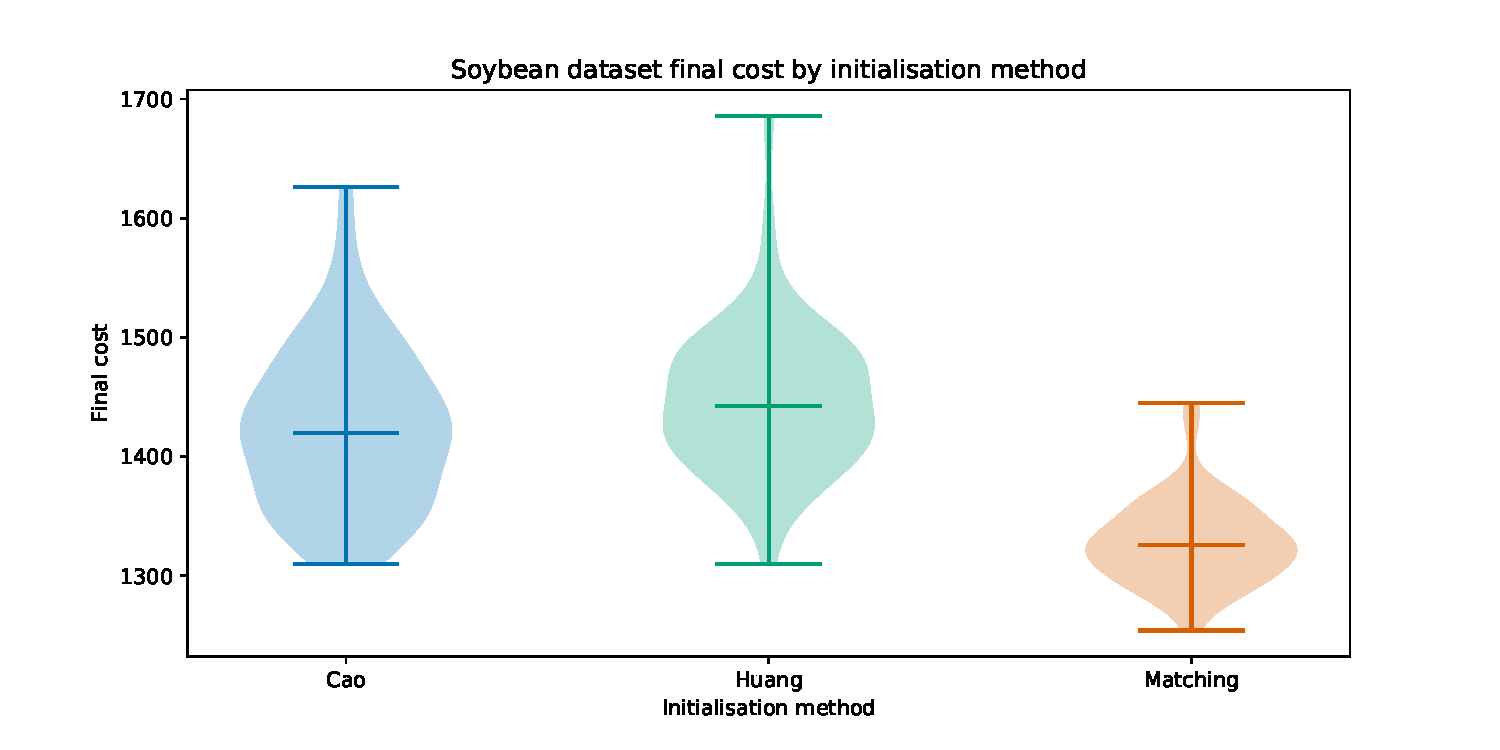
\includegraphics[width=\imgwidth]{%
        img/soybean_final_cost_violinplot.pdf%
    }\caption{Distribution of final cost by initialisation for the soybean
              dataset.}
\end{figure}

\begin{figure}
    \centering
    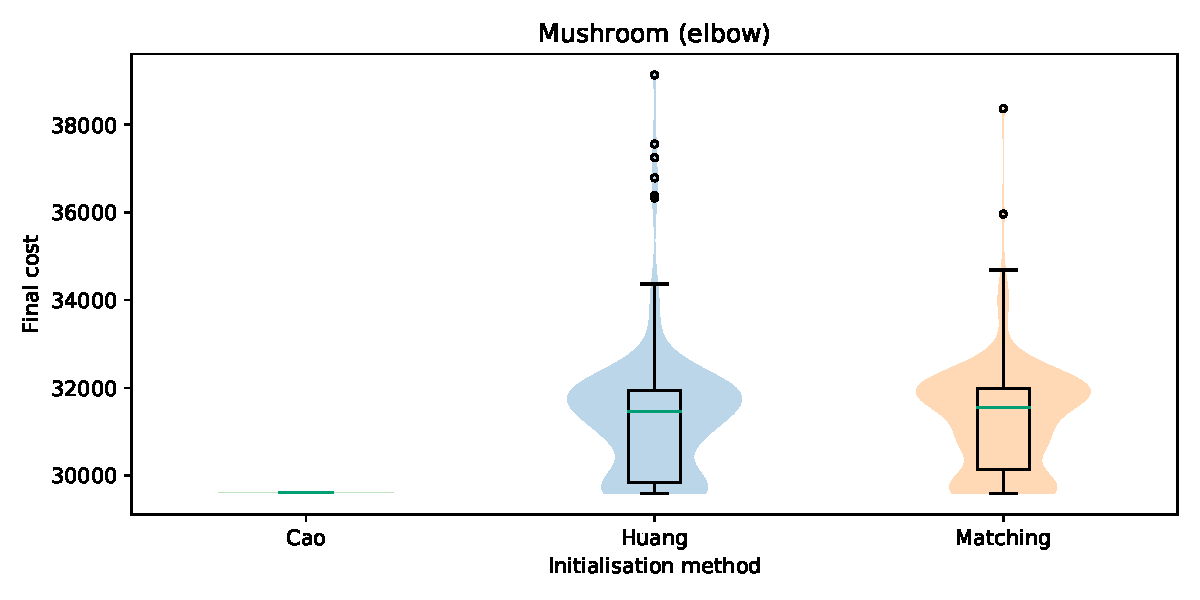
\includegraphics[width=\imgwidth]{%
        img/mushroom_final_cost_violinplot.pdf%
    }\caption{Distribution of final cost by initialisation for the mushroom
              dataset.}
\end{figure}

\begin{figure}
    \centering
    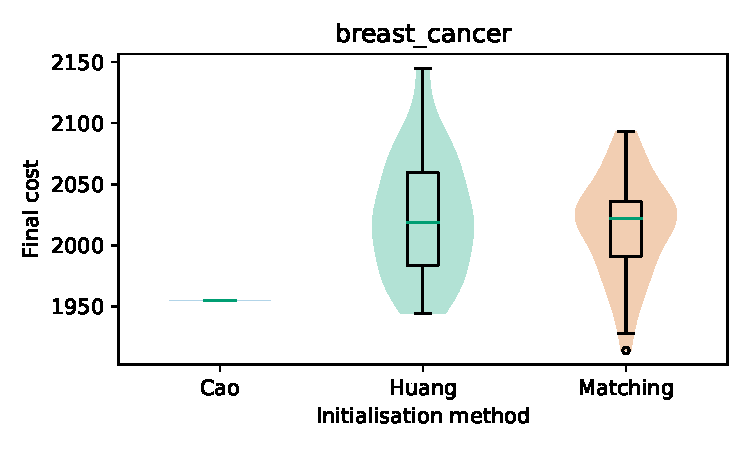
\includegraphics[width=\imgwidth]{%
        img/breast_cancer_final_cost_violinplot.pdf%
    }\caption{Distribution of final cost by initialisation for the breast
              cancer dataset.}
\end{figure}

\begin{figure}
    \centering
    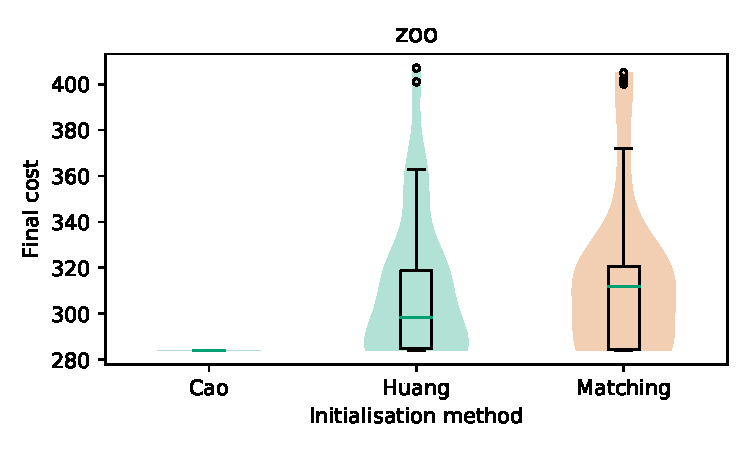
\includegraphics[width=\imgwidth]{%
        img/zoo_final_cost_violinplot.pdf%
    }\caption{Distribution of final cost by initialisation for the zoo animal
              dataset.}
\end{figure}


\begin{figure}
    \centering
    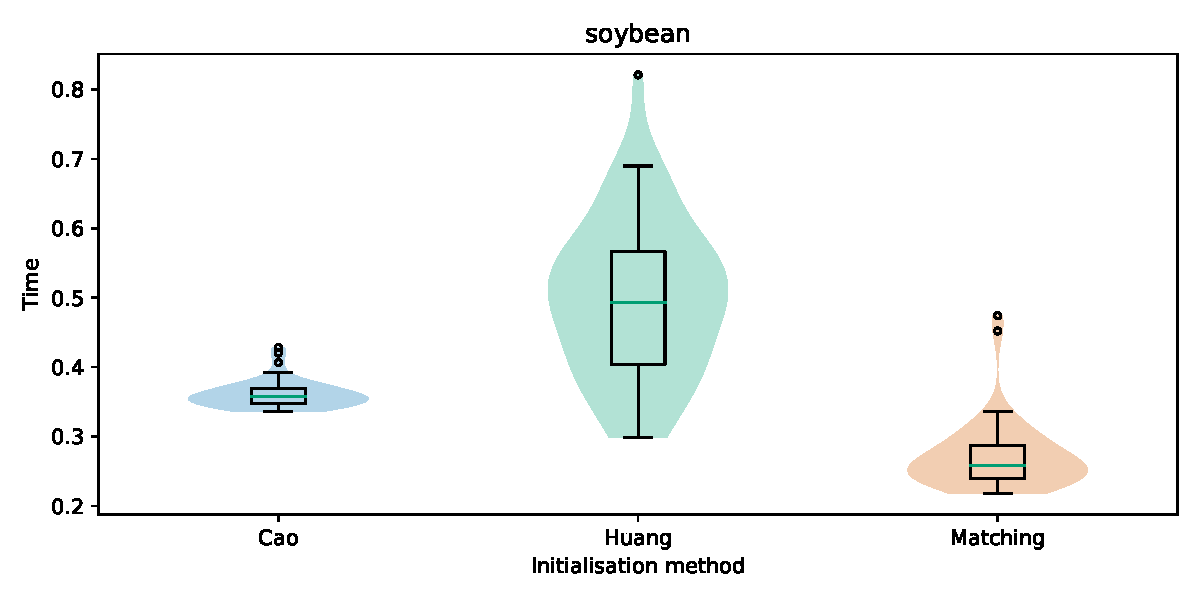
\includegraphics[width=\imgwidth]{%
        img/soybean_time_violinplot.pdf%
    }\caption{Distribution of time taken by initialisation for the soybean
              dataset.}
\end{figure}

\begin{figure}
    \centering
    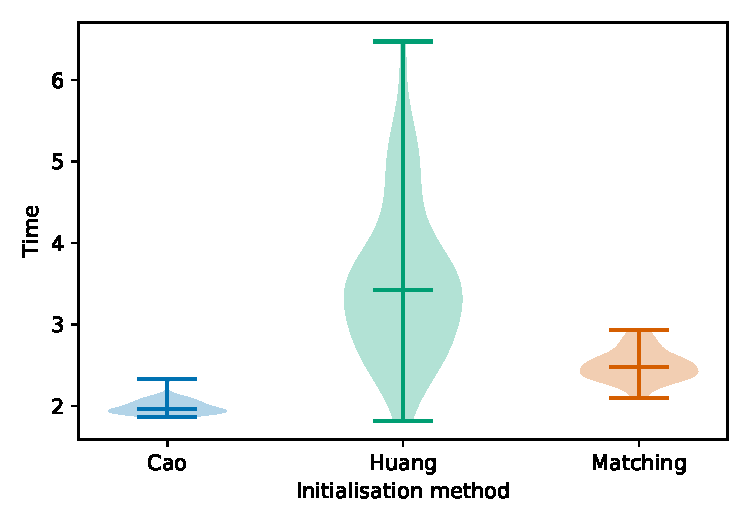
\includegraphics[width=\imgwidth]{%
        img/mushroom_time_violinplot.pdf%
    }\caption{Distribution of time taken by initialisation for the mushroom
              dataset.}
\end{figure}

\begin{figure}
    \centering
    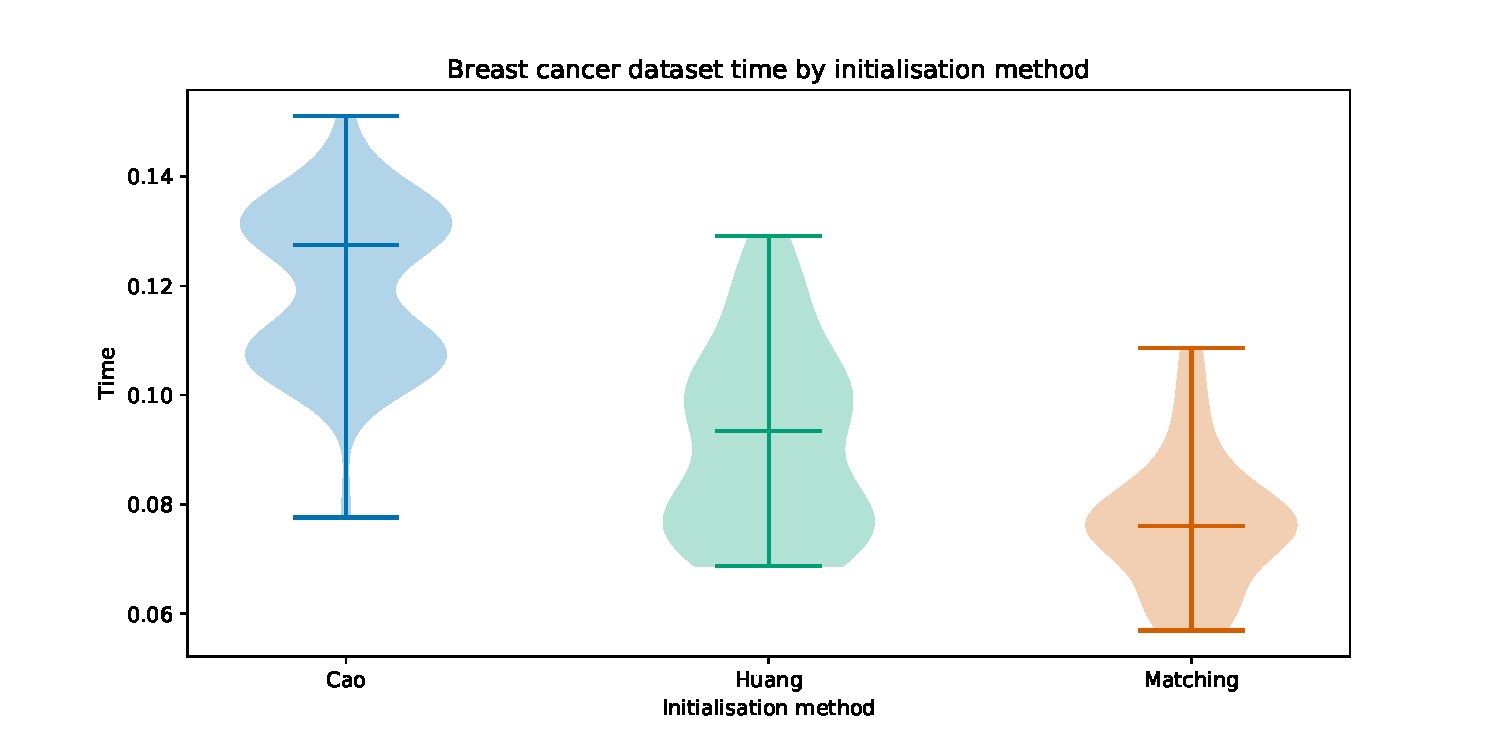
\includegraphics[width=\imgwidth]{%
        img/breast_cancer_time_violinplot.pdf%
    }\caption{Distribution of time taken by initialisation for the breast
              cancer dataset.}
\end{figure}

\begin{figure}
    \centering
    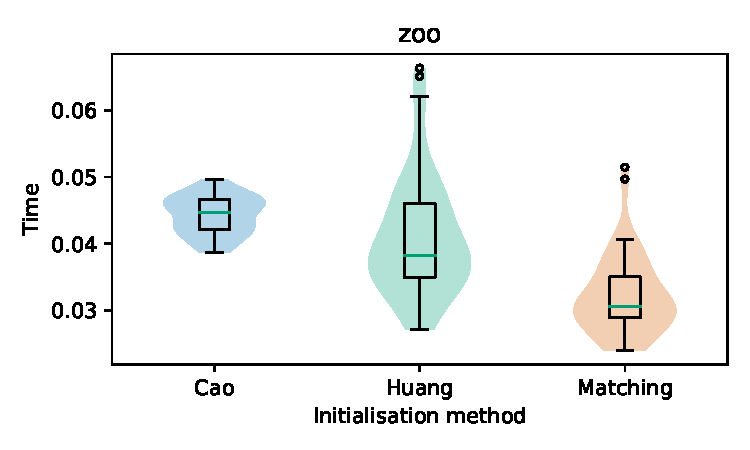
\includegraphics[width=\imgwidth]{%
        img/zoo_time_violinplot.pdf%
    }\caption{Distribution of time taken by initialisation for the zoo animal
              dataset.}
\end{figure}
